\documentclass[12pt,runningheads]{article}
\usepackage[utf8]{inputenc}
\usepackage{amsmath,amssymb,hyperref,array,xcolor,multicol,verbatim,mathpazo}
\usepackage[normalem]{ulem}
\usepackage[pdftex]{graphicx}
\begin{document}

%%%% In most cases you won't need to edit anything above this line %%%%

\title{Assignment 3: Bayesian Well-Log Analysis\\GPGN 409}
\author{Garrett Sickles}
\maketitle
\pagebreak
\begin{enumerate}
\item \textit{What are the model and data parameters?}\\ \\ 
The data parameters are the porosity and density and the model parameter is the P-wave velocity.
\item \textit{Construct the prior joint probability density based on the observed values of $\phi$ and $\rho$ and for a P-wave velocity related to the GR log by the relation
\begin{align*}
v_{p}\ =\ 5.654 - 0.008\ GR
\end{align*}
Specify what distribution you are using and justify your choice of parameters defining your chosen distributions.\\Assume that a-priori all variables are independent.}\\ \\
The prior joint probability distribution appears in the figures below in two forms, a sliced volume and a projected volume.
\begin{figure}[!h]
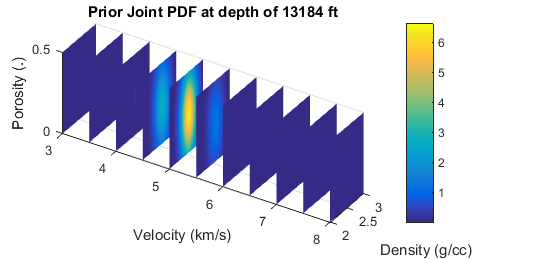
\includegraphics[width=\textwidth]{PriorS.png}
\end{figure}
\begin{figure}[!h]
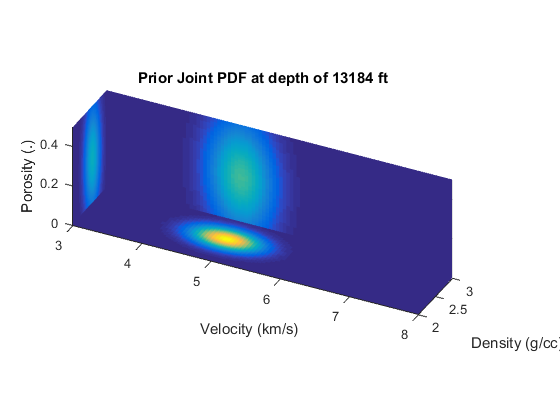
\includegraphics[width=\textwidth]{PriorP.png}
\end{figure}
I used a three dimensional independent Gaussian distribution to create the volume slice in the two previous figures. The equation used to implement this distribution was
\begin{align*}
f(\vec{x},\vec{\mu},\Sigma)\ =\ \frac{1}{\sqrt[]{|\Sigma|(2\pi)^{d}}}\ e^{-\frac{1}{2}(\vec{x}-\vec{\mu})^{\top}\Sigma^{-1}(\vec{x}-\vec{\mu})}
\end{align*}
where $\vec{x}$ and $\vec{\mu}$ are of length $d$ and $\Sigma$ is a $d$ by $d$ symmetric matrix of the form
\begin{align*}
\Sigma\ =
\begin{bmatrix}
\ \sigma(\vec{v})\ &\ 0\ &\ 0\ \ \\ \\
\ 0\ &\ \sigma(\vec{\rho})\ &\ 0\ \ \\ \\
\ 0\ &\ 0\ &\ \sigma(\vec{\phi})\ \
\end{bmatrix}
*\frac{|caliper(depth)\ -\ 6.000|}{range(caliper(...))}\\
\end{align*}
such that $\sigma$ is the standard deviation of a one dimensional data set and the function $caliper$ returns the caliper measurement at a given depth.\\ \\
I chose to use the standard deviations and the percent difference of the caliper from what it should be because I believe through testing and my understanding of the problem that this adequately scales the distribution to reflect the accuracy of the velocity estimate at depth. This incorporates information from two essential distributions, the caliper thickness at a measurement's given depth and the total distribution of each given data parameter in question.

\pagebreak
\item \textit{Construct the theoretical joint probability density assuming uncertainty relative to the theoretical prediction. Specify what distribution you are using and justify your choice of parameters defining your chosen distributions.}\\ \\
The theoretical joint probability distribution appears in the figures below in two forms, a sliced volume and a projected volume.

\begin{figure}[!h]
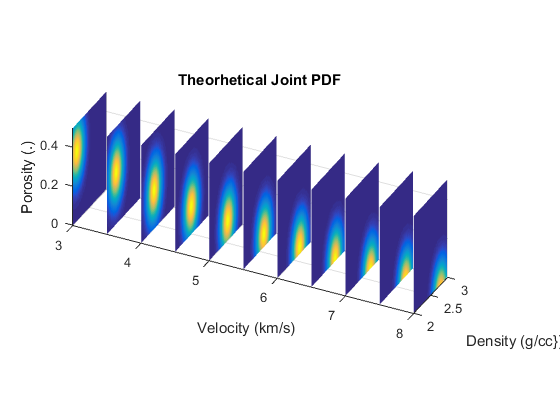
\includegraphics[width=\textwidth]{TheoryS.png}
\end{figure}
\begin{figure}[!h]
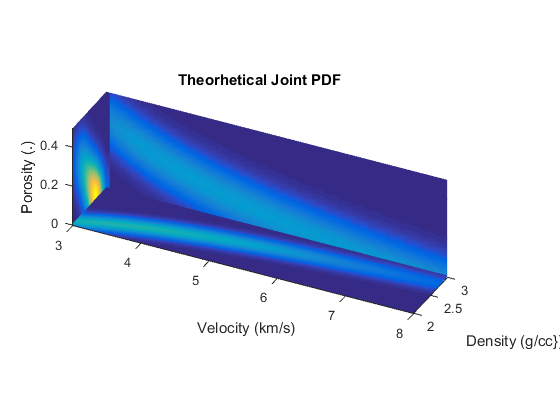
\includegraphics[width=\textwidth]{TheoryP.png}
\end{figure}
I made my theoretical joint pdf's by using the equations
\begin{align*}
\frac{1}{v}\ =\ \frac{1\ -\ \phi}{v_{M}}\ +\ \frac{\phi}{v_{F}}\ ,\ \rho\ =\ (1\ -\ \phi)\rho_{M}\ +\ \phi\rho_{F}
\end{align*}
to get a three dimensional point of the form $(v,\rho,\phi)$ at any given value of one of the three variables. Iterating across the range of the velocities, I inserted slices representing a two dimensional Gaussian distribution on the other two variables to assemble the three dimensional volume. Instead of defining my sigma matrix as in the prior joint pdf, I chose to define it as a diagonalization of the order of magnitude of the standard deviation of the various parameters, respectively.
\pagebreak
\item \textit{Construct the posterior joint probability density based on the prior and theoretical pdf's.}\\ \\
The posterior joint probability distribution appears in the figures below in two forms, a sliced volume and a projected volume.
\begin{figure}[!h]
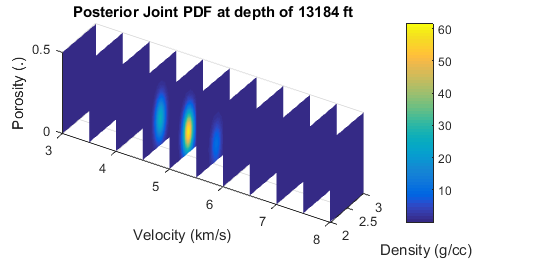
\includegraphics[width=\textwidth]{PostS.png}
\end{figure}
\begin{figure}[!h]
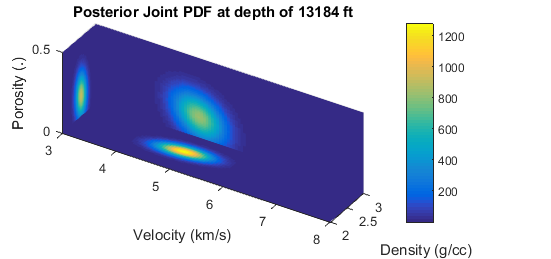
\includegraphics[width=\textwidth]{PostP.png}
\end{figure}
These figure represent the three dimensional element wise multiplication of the prior joint pdf with the theorhetical joint pdf.
\pagebreak
\item \textit{Compare the model prior and posterior PDFs and explain the observed differences.}
\end{enumerate}
\end{document}